\subsection{Retrieval} \label{sec:Retrieval}
\begin{figure}[t]
    \centering
    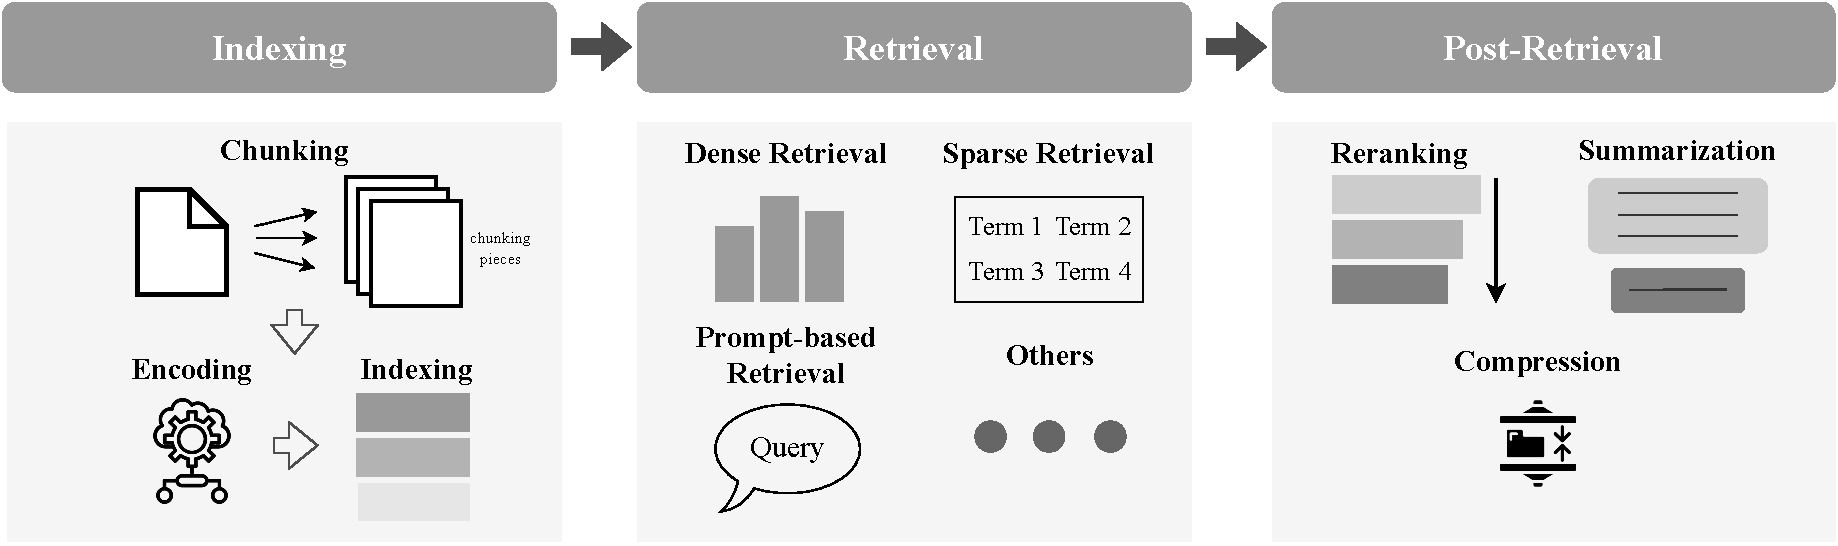
\includegraphics[width=\linewidth]{figures/retrieval.pdf}
    \caption{Overview of the personalized retrieval stage.}
    \label{fig:retrieval}
\end{figure}
\subsubsection{\textbf{Definition}}

The retrieval process involves finding the most relevant documents $D^*$ from a corpus $\mathcal{C}$ based on a query $q^*$, as shown in Figure~\ref{fig:retrieval}. To incorporate personalization, additional user-specific information $p$ is integrated into the retrieval function  $\mathcal{R}$. This allows the retrieval process to tailor the selected documents to align with individual user preferences or contexts, thereby enhancing the relevance and personalization of the generated outputs.
\begin{equation}
D^* =  \mathcal{R}\left(q^*,\mathcal{C},p\right)
\end{equation}

In the retrieval process, personalization can primarily be introduced by focusing on three steps: indexing, retrieval, and post-retrieval. These steps ensure efficient and accurate retrieval of relevant documents or knowledge, while tailoring the process to individual user preferences. Below, we provide a detailed explanation of each step.

\subsubsection{\textbf{Indexing}}
Indexing organizes knowledge base data into a structured format to facilitate efficient retrieval. Within the RAG pipeline, documents are either chunked or entirely encoded into representations before being integrated into searchable systems~\cite{douze2024faiss, annoy}. Conventional encoding methods employ either sparse encoding techniques (\eg TF-IDF~\cite{rajaraman2011mining}, BM25~\cite{robertson2009probabilistic}) or dense encoding approaches leveraging pre-trained models, such as BERT~\cite{koroteev2021bert}, Siamese Encoders~\cite{reimers2019sentence}, or LLM-based encoders~\cite{li2023towards, xiao2024c}.

To introduce personalization at the indexing stage, PEARL~\cite{mysore2023pearl} generates user embeddings by encoding personal history data with models like DeBERTa. These embeddings are subsequently clustered to create personalized shared indices. Other approaches integrate knowledge graphs into indexing to enhance retrieval performance. For example, KG-Retriever~\cite{chen2024kg} employs a Hierarchical Index Graph, consisting of a knowledge graph layer and a collaborative document layer, to improve RAG retrieval. EMG-RAG~\cite{wang2024crafting} incorporates personalized memory within an editable knowledge graph, enabling dynamic retrieval. Similarly, PGraphRAG~\cite{au2025personalized} leverages user-centric knowledge graphs to enhance personalization in retrieval tasks.


\subsubsection{\textbf{Retrieval}}
The Retrieval step matches a user query with the indexed knowledge base to fetch relevant candidates. It can be broadly categorized into four different types: (1) Dense Retrieval,  (2) Sparse Retrieval, (3) Prompt-based Retrieval, and  (4) Others.

\paragraph{\textbf{\textit{{(1). Dense Retrieval.}}}}
Dense retrieval methods often use vector embeddings and similarity metrics (\eg cosine similarity) and achieve personalization by encoding user preferences, context, or interactions into query or document embeddings, enabling tailored results through similarity-based matching. For instance, MeMemo \cite{wang2024mememo} retrieves personalized information by matching user-specific embeddings with document vectors, focusing on private, on-device text generation. Similarly, RECAP \cite{liu2023recap} and LAPDOG \cite{huang2024learning} enhance personalized dialogue generation by encoding queries and user profiles as dense vectors and retrieving top-N results, ensuring user-specific context drives the responses. In chatbots, \citet{gu2021partner} integrates conversational context and user profiles to align retrieved responses with user personas. PersonaLM \cite{mathur2023personalm} employs group-wise contrastive learning, training its retrieval model to align user queries with domain-specific text fragments, thereby improving personalization. UIA \cite{zeng2023personalized} employs dual encoders to retrieve documents tailored to user preferences. XPERT \cite{vemuri2023personalized} incorporates temporal events and user interactions into embeddings, enabling large-scale retrieval across millions of items.

Dense retrieval also enhances specific applications like e-commerce, medical assistance, and language models. DPSR \cite{zhang2020towards} and RTM \cite{bi2021learning} encode user queries and product information to personalize product searches dynamically. Pearl \cite{mysore2023pearl} and MemPrompt \cite{madaan2022memory} retrieve personalized content by leveraging historical user data and memory-assisted mechanisms. ERRA \cite{cheng2023explainable} uses review embeddings as dense queries for recommendations. In medical assistance, MALP \cite{zhang2023llm} and USER-LLM \cite{ning2024user} integrate short- and long-term user interactions into embeddings for contextualized, personalized responses. Finally, PER-PCS \cite{tan2024personalized} retrieves relevant information using individual user histories, enhancing the personalization capabilities of large language models.  

\paragraph{\textbf{\textit{{(2). Sparse Retrieval.}}}}
Sparse retrieval methods often rely on term-based matching (\eg BM25) and apply personalization by assigning higher weights to terms or keywords that are more relevant to the user.  OPPU \cite{tan2024democratizing} uses the BM25 algorithm to select the k most relevant records from the user's historical data for the current query. Similarly, PAG \cite{richardson2023integrating} incorporates user input and profiles to enhance summarization and retrieval, aligning sparse representations with personalization objectives for large language models. \citet{au2025personalized} uses BM25 search algorithms to find entries related to the target user or neighboring users through the graph structure. UniMS-RAG \cite{wang2024unims} combines sparse and dense retrieval by leveraging multi-source knowledge, such as dialogue context and user images, to refine personalized responses in dialogue systems. Lastly, \citet{deng2022toward} apply sparse retrieval to support fact-based queries, considering user queries and preferences to enhance answer generation for e-commerce applications. 

\paragraph{\textbf{\textit{{(3). Prompt-based Retrieval.}}}}
Prompt-based retrieval leverages prompts to guide retrieval from the model or external sources and introduces personalization by crafting user-specific prompts that guide the retrieval process. These prompts may include explicit user preferences, historical interactions, or detailed instructions that reflect the user’s unique requirements. By embedding this personalized context directly into the prompt, the retrieval process can dynamically adjust to capture and return results that are most relevant to the user. LAPS \cite{joko2024doing} focuses on multi-session conversational search by storing user preferences and dialogue context, then using prompts to retrieve relevant information tailored to the user's biases and categories of interest. UniMP \cite{wei2024towards} employs user interaction histories as input to prompt-based retrieval, enabling personalized recommendations for multi-modal tasks, such as vision-language applications, by aligning prompts with user behavioral data. In contrast, \citet{shen2024heart} explores the use of LLMs to extract empathy and narrative styles from user-provided stories, but this work primarily focuses on style extraction and does not explicitly involve a retrieval component. 

\paragraph{\textbf{\textit{{(4). Others.}}}}
Reinforcement learning-based retrieval personalizes the process by optimizing retrieval policies based on user feedback, learning user preferences over time to adjust strategies. \citet{salemi2024optimization} combines models like BM25, RbR, and dense retrieval, refining them with reinforcement learning (RL) and knowledge distillation (KD) to adapt to user profiles for personalized outputs. Parameter-based retrieval leverages pre-trained model parameters to implicitly store and retrieve user-specific information, allowing direct retrieval from the model without traditional indices. PersonalTM \cite{lian2023personaltm} generates document identifiers (Document IDs) using a Transformer model, encoding query, history, and document relationships into its parameters for personalization. Similarly, \citet{zhang2024personalized} uses parameterized representations to integrate user queries and histories, tailoring responses to individual preferences.

\subsubsection{\textbf{Post-retrieval}}
Current Post-Retrieval methods primarily focus on refining retrieved documents or responses to improve relevance and coherence, current methodologies could be categorized into three parts (1) Re-ranking, (2) Summarization, and (3) Compression.

\paragraph{\textbf{\textit{{(1). Re-ranking.}}}}
Re-ranking enhances personalized content generation by prioritizing more relevant documents at the top. PersonaRAG~\cite{zerhoudi2024personarag} extends RAG by integrating user-centric agents, such as the Live Session Agent and the Document Ranking Agent, to refine document ranking and improve overall performance. \citet{pavliukevich2024improving} propose a cross-encoder BERT model for re-ranking external knowledge within a personalized context. UniMS-RAG~\cite{wang2024unims} introduces a scoring mechanism that evaluates retrieved documents and outputs by optimizing the retriever. Besides, it includes an evidence attention mask, enabling re-ranking during inference and applying it to personalized datasets. ~\citet{salemi2024learning} present an iterative approach to optimizing ranking results based on the expectation-maximization algorithm, with performance validated in personalized scenarios.


\paragraph{\textbf{\textit{{(2). Summarization.}}}}
Summarization refers to the process of summarizing retrieved information to enhance performance. For instance,~\citet{zhang2025rehearse} introduced a role-playing agent system to summarize retrieved history in order to improve the final Personalized Opinion Summarization process.

\paragraph{\textbf{\textit{{(3). Compression.}}}}
Compression involves condensing embeddings or retrieved content to enhance efficiency and effectiveness. Approaches like AutoCompressor~\cite{chevalier2023adapting} compress contextual embeddings into shorter semantic representations, and FIT-RAG~\cite{mao2024fit} introduces a self-knowledge recognizer along with a sub-document-level token reduction mechanism to minimize tokens within RAG pipeline. However, few studies have specifically explored personalized fields, highlighting a promising direction for future research.

\subsubsection{\textbf{Discussion}}
Indexing, retrieval, and post-retrieval methods each play a critical role in ensuring efficient and personalized information processing, with specific applications and trade-offs. Indexing focuses on organizing knowledge bases for efficient retrieval, using techniques such as sparse encoding methods like TF-IDF and BM25, which are efficient but limited in understanding semantics, and dense encoding methods like BERT and DeBERTa, which provide better semantic understanding but require significant computational resources. These methods are widely used in tasks like question answering and personalized recommendation systems. Retrieval involves matching user queries with relevant documents and can be categorized into dense retrieval, which provides high semantic understanding and personalization but is computationally expensive; sparse retrieval, which is efficient and interpretable but less capable of handling semantics; prompt-based retrieval, which is highly flexible and adaptable to user needs but requires careful engineering of prompts; and advanced methods like reinforcement learning-based approaches, which dynamically adapt to user feedback but are complex to implement. This step is essential in applications like personalized dialogue systems, search engines, and e-commerce. Post-retrieval methods refine retrieved results to enhance relevance and coherence through re-ranking, which improves personalization and prioritizes relevant content but increases computational overhead; summarization, which simplifies complex information for better user understanding but risks losing critical details; and compression, which reduces computational costs by condensing information but remains underexplored in personalized contexts. Together, these methods provide a comprehensive pipeline for delivering efficient, relevant, and personalized outputs, balancing their strengths in semantic understanding, relevance, and flexibility with challenges related to computational costs and implementation complexity.